\chapter{Evaluation}
\label{Evaluation}

\section{Evaluating the system performance of the software architecture}

%SeNAmI start
\subsection{Related work}
The two M3-based smart space implementations described in Section \ref{m3} were evaluated by Etel\"aper\"a et al \cite{Etelapera2011}. They performed both a qualitative evaluation and quantitative measurements. The performance measurements were made on a Intel Atom 1.6GHz laptop connected via a 100Mbps Ethernet router to a Intel Pentium M 1.7GHz laptop. The qualitative evaluation focused on documentation, installation process and portability as well as run-time usability. According to \cite{Etelapera2011} RIBS is up to 237 times faster than Smart-M3 in certain instances, but that its memory model limits the number of use cases it can be applied to. RIBS uses static memory allocation (with no disk storage) and a bitcube triple store, which means that the maximum number of triples have to be known a priori.

Query time measurements for Smart-M3 indicated a query time of 4.4ms for one triple and 8.6ms for 10 triples. For RIBS a query time of 0.65ms were measured for one triple. RIBS did not support querying 10 triples at the time the evaluation was performed. Subscription time measurements indicated a subscription indication time of 140ms for Smart-M3, while RIBS measured 0.75ms.

\cite{Bhardwaj2011} did a performance analysis based on end-to-end delay measurements between the smart objects in smart spaces. The analysis shows that the end-to-end delays are mostly dominated by KP-to-SIB updates, rather than the processing delays on KPs or on the SIB.

% A number of ontologies have been developed for ubiquitous computing environments. Chen et al. \cite{chen2004} defined SOUPA, a context ontology based on OWL (Web Ontology Language), to support ubiquitous agents in their Context Broker Architecture (CoBrA). The ontology supports describing devices on a very basic level (e.g. typical object properties are \texttt{bluetoothMAC} or \texttt{modelNumber}), but it has no explicit support for modeling more general device capabilities.

% Ngo et al. \cite{Ngo2004} developed the CAMUS ontology in OWL to support context awareness in ubiquitous environments. Their device ontology is based on the FIPA device ontology specification\footnote{http://www.fipa.org/specs/fipa00091/SI00091E.html}. Unfortunately it does not define a notion of completeness, and the ontology is thus not considered generic enough for general use in ubicomp environments.

Luukkala et al \cite{Luukkala2010} used Smart-M3 with Answer Set Programming (ASP) techniques to handle resource allocation and conflict resolution. They used the SPICE Mobile Ontology\footnote{http://ontology.ist-spice.org/} to describe device capabilities and ASP as a rule-based approach to reasoning. The SPICE ontology allows for the definition of device capabilities in a sub-ontology called Distributed Communication Sphere (DCS) \cite{Villalonga2009}. %While the ontology provides for a detailed description of the different modality capabilities, e.g. being able to describe force feedback as a \texttt{TactileOutputModalityCapability}, there are no subclass assertions made for other device capabilities.

%This could be extended with work from Riboni et al; Liming Chen (and maybe Sabou's paper)

\subsection{Implementation}
\label{implementation}

The software framework that was used to implement the system is based on the SOFIA IOP. SOFIA\footnote{http://www.sofia-project.eu/} (Smart Objects For Intelligent Applications) is an European research project within the ARTEMIS framework that attempts to make information in the physical world available for smart services - connecting the physical world with the information world. The SOFIA IOP uses a blackboard architectural model that implements the ideas of space-based computing \cite{Honkola2010}. It consists of two main components: a SIB (Semantic Information Broker) that acts as a common, semantic-oriented store of information and device capabilities, and KPs (Knowledge Processors), virtual and physical smart objects that interact with one another through the SIB. Various SIB implementations exist that conform to the M3 specification, of which Smart-M3 was the first open source reference implementation released in 2009\footnote{http://sourceforge.net/projects/smart-m3/}. RIBS (RDF Information Base System) is a C-based implementation of M3 targeted for devices with low processing power, but requires a high amount of memory \cite{Etelapera2011}.  The SIB implementation used in the pilot is called ADK-SIB (Application Development Kit SIB) and was developed within the SOFIA project. 

%The system architecture of the implementation of the smart home pilot is shown in Figure \ref{pilot}.
The smart home pilot follows the following scenario:

\textit{Mark and Dries enter their home. The intelligent lighting system (Presence KP) detects their presence, and switches the lights on, and notifies the smart space about user presence. The decorative wall-wash lights (Lamp KP) are in turn notified of user presence by the smart space, and turn themselves on. Mark and Dries start listening to music (Music Player KP). They would like to try to render the music on a lighting device to also create some visual effects accompanying the music. They query the smart space and find out that the lighting device can render these light effects (using the Sound/Light Transformer KP). They make a connection between the music player and the lighting device using the Connector (Connector KP). The light is rendered on the lighting device. To put the focus on the lighting device, the decorative wall-wash lights in the room automatically dim themselves down. At the same time, the light pattern also starts being rendered on the remote lighting device, where Mark's sister Sofia can observe the same light effects in her own house.}

\textit{At another location: after a while, Sofia is curious and wants to listen to the music that Mark and Dries are listening to. She connects her lighting device to her stereo, and the same song plays on her surround sound system (remote Music Player KP).}
% --Note: Since we don't mention spotlight navigation elsewhere, Sachin suggested we remove it from the scenario

%She uses the spotlight navigation device to make a connection from the bonding device to the stereo. When she starts using the spotlight navigator, the lights in the room dim down to enhance the visibility of the spotlight. Once the connection is made, the lights go back up.


% \begin{figure}
% \centering
% \includegraphics[width=250px]{pilot}
% \caption{System architecture of the Smart Home Pilot}
% \label{pilot}
% \end{figure}

In the smart home pilot, media content is shared among several devices in a smart home setting. Music is shared between a mobile device, a stereo speaker set and a lighting device that renders the mood of the music with colored lighting. The music experience, consisting of both light and music information, is also shared remotely between friends living in separate homes through the lighting device. Other lighting sources, like the smart functional lighting and the smart wall wash lights are sensitive to user presence and the use of other lighting sources in the environment.

The performance measurements were made in an environment that approximates a real-world home environment for these kinds of devices. Two wireless routers were placed in two different locations (Home A and B), bridged with an ethernet network cable. One router was configured to act as a DHCP server, while the other acted as a network bridge. The Sound/Light Transformer (SLT) KP was connected to the router in Home B, while the Connector KP, Music Player KP and SIB were connected to the router in Home A. All components were connected to the network via the 802.11g wireless protocol. The system specifications of each component used in the performance evaluation is shown in Table \ref{specs}.

\begin{table*}[!t]
\caption{System specifications of components used in measurement evaluation}
\label{specs}
\centering
\begin{tabular}{|l|l|l|l|l|}
\hline
Component & CPU & Operating system & Memory & Programming Language \\
\hline
Semantic Information Broker (SIB) & Intel Core 2 Duo 2.8GHz & Ubuntu Linux 10.04 & 4GB & Java \\
Sound/Light Transformer KP & Intel Core 2 Duo 2.2GHz & Ubuntu Linux 11.04 & 2GB & Java\\
Connector KP & Intel Core 2 Duo 2.6GHz & Mac OS X 10.6.8 & 4GB & Python\\
Music Player KP & OMAP 3430 ARM Cortex-A8 & Maemo Linux 5 & 256MB & Python\\
Presence KP  & Intel Pentium M & Ubuntu Linux 10.04 & 512MB & Python\\
Lamp KP  & Intel Pentium M & Ubuntu Linux 10.04 & 512MB & Python\\
\hline
\end{tabular}
\end{table*}

Figure \ref{soundLight} and Figure \ref{connectorseq} show the sequence diagrams of the measurements made for the SLT KP and the Connector KP respectively. During the pilot, 86 measurements were made by the SLT KP (each time an event was received), and 961 measurements were made by the Connector KP (each time a user scans a tag).

\begin{figure}
\centering
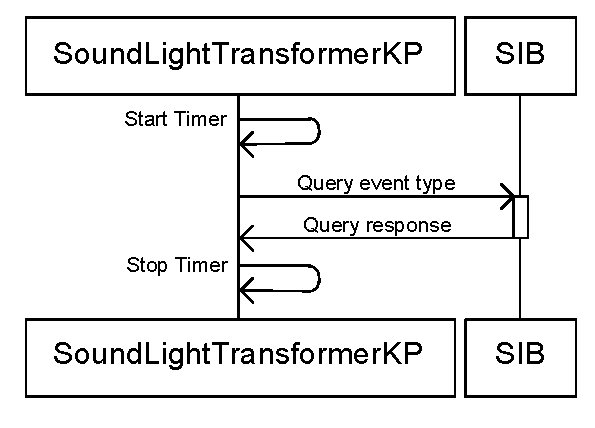
\includegraphics[width=150px]{soundLight}
\caption{Sequence diagram of Sound/Light Transformer KP query measurement}
\label{soundLight}
\end{figure}

\begin{figure}
\centering
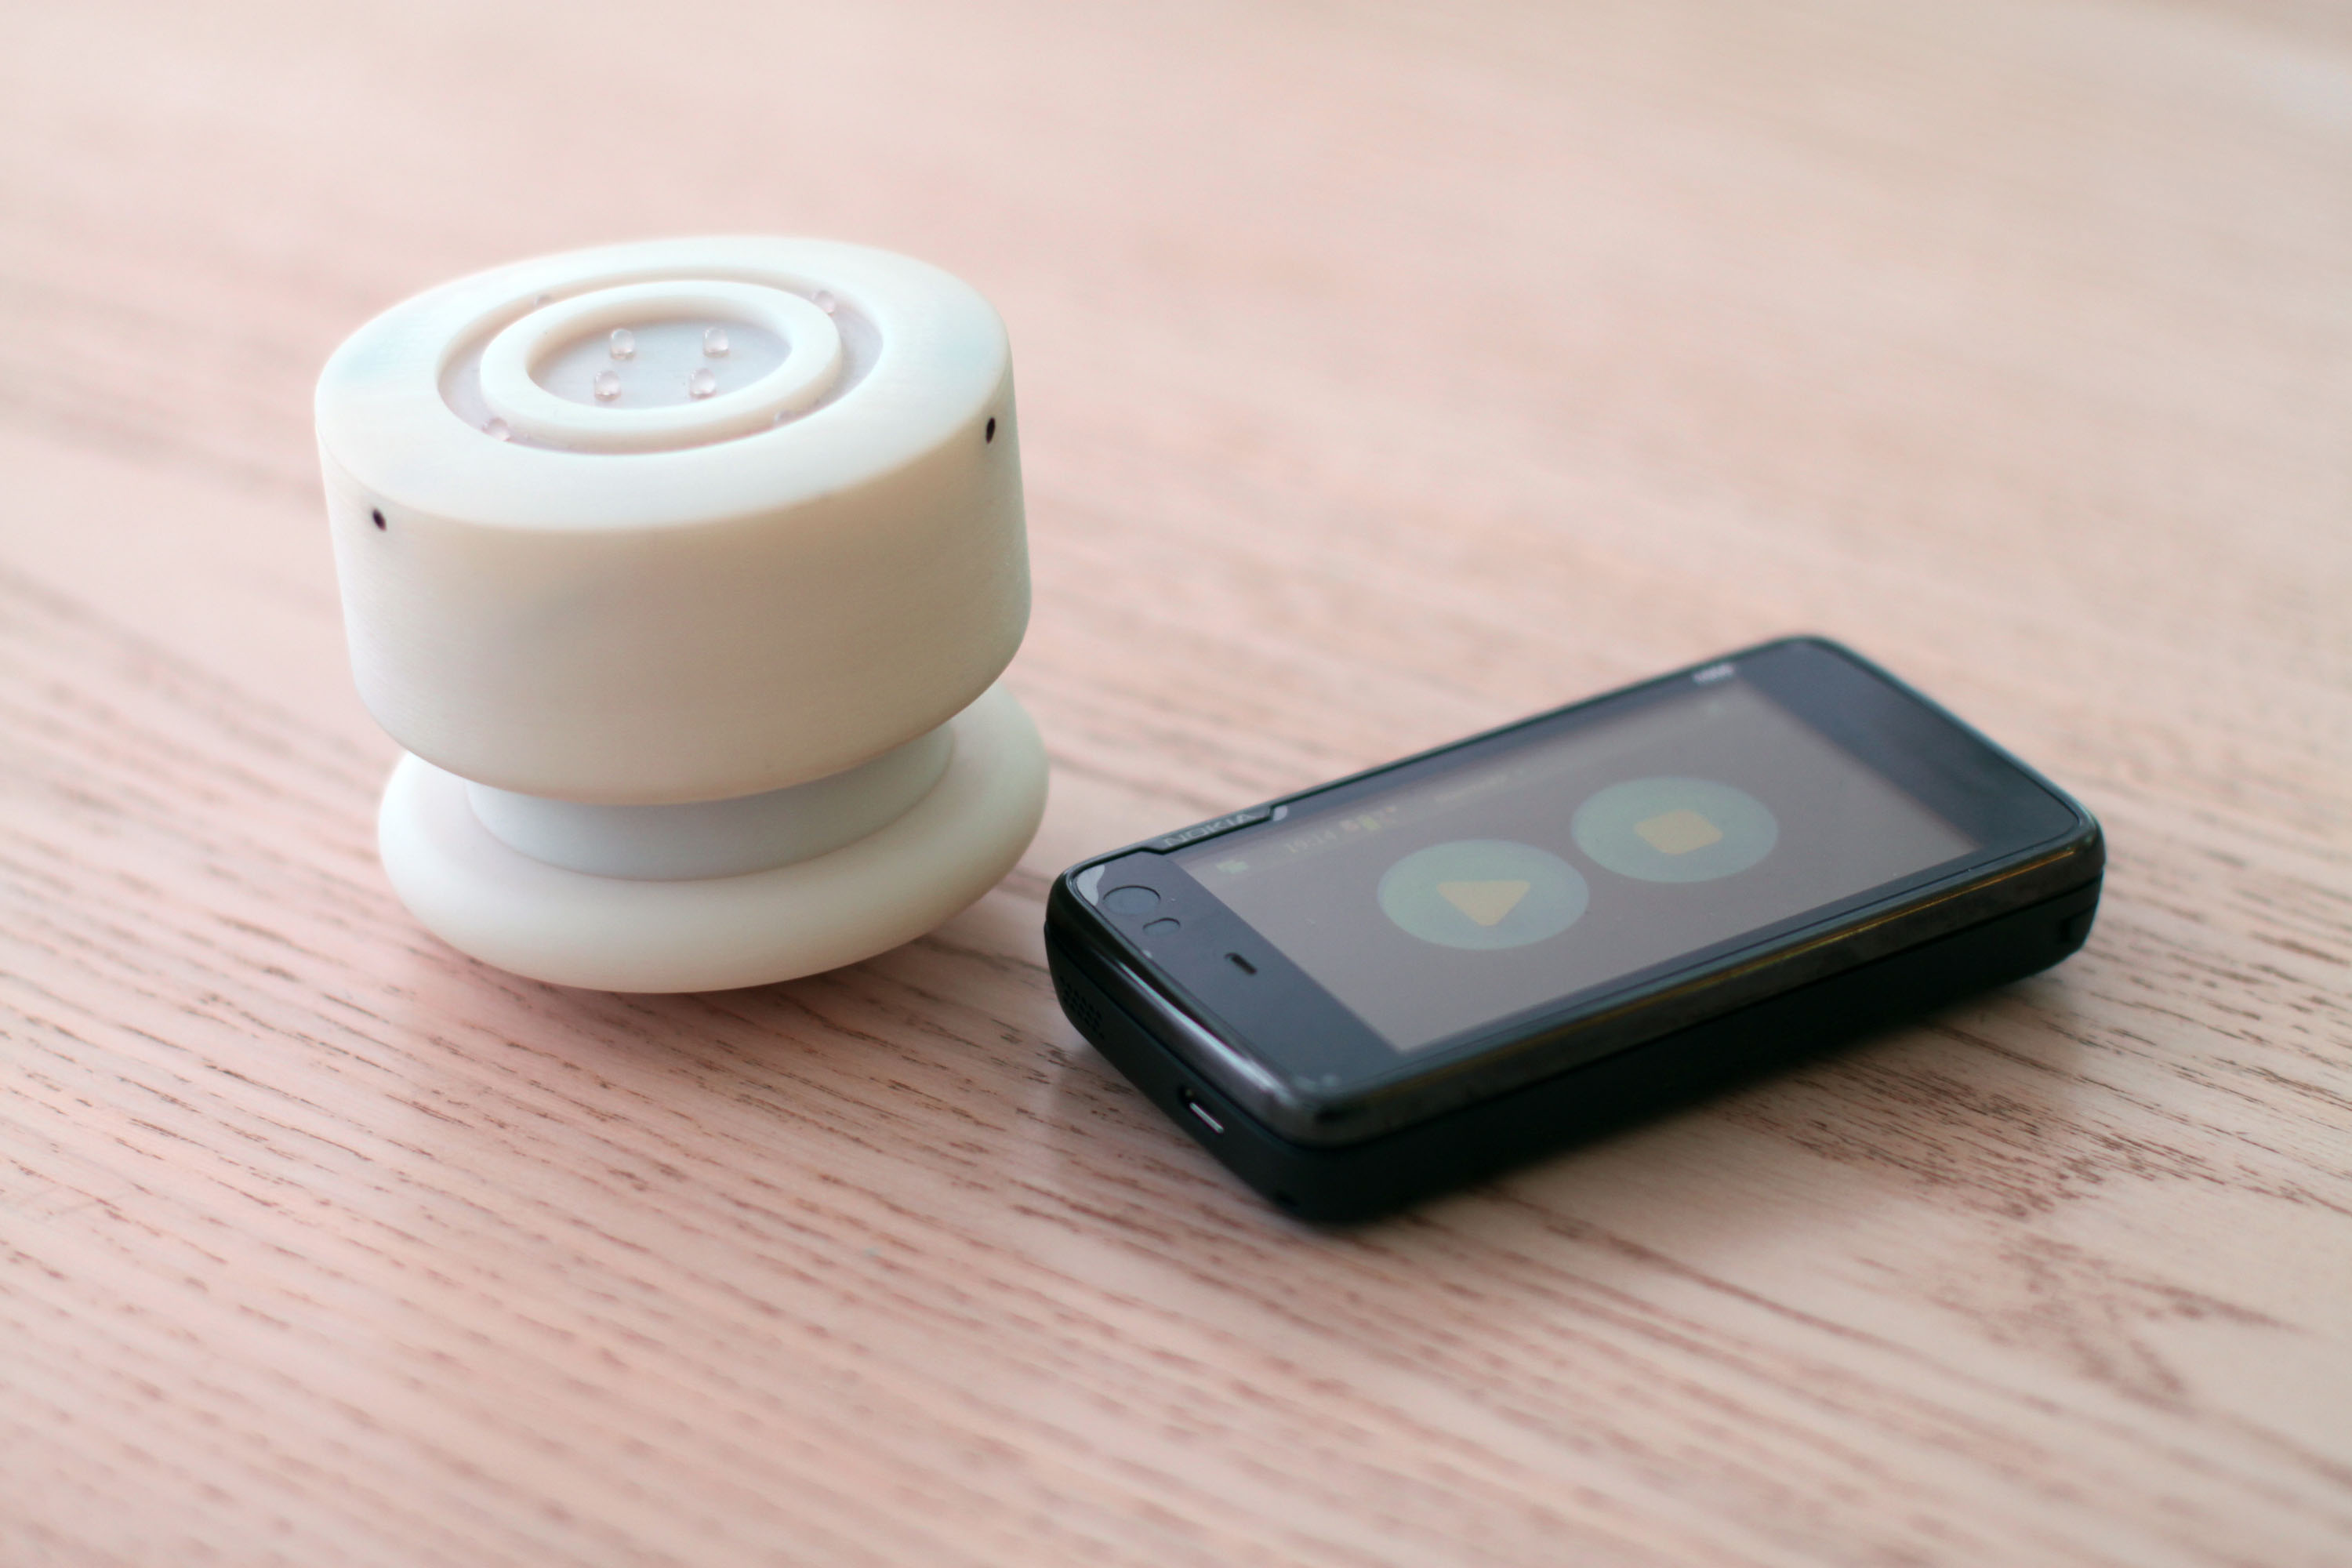
\includegraphics[width=150px]{connector}
\caption{Sequence diagram of Connector KP query measurement}
\label{connectorseq}
\end{figure}

For the music player KP, we measured the time between inserting a new event, and receiving an update from the SIB indicating that the specific event had occurred. First a subscription is made to the \texttt{PlayEvent} type, as seen in Figure \ref{N900}. A new \texttt{PlayEvent} is generated by the KP, and when the KP is notified of this event by the SIB, the KP queries the SIB to determine if the notification is indeed for the event that it generated itself.

The Lamp-KP was connected to the decorative wall-wash lights (four LED lamps), creating colored illumination on the wall of the room. The lamps are shown in Figure \ref{lamp-KP}, including a description of its components. The Presence KP (P-KP) determines the presence of a user in an activity area of a room and sends the presence information to the SIB. The Lamp-KP is subscribed to this presence information, and gets updated whenever the presence is updated by the P-KP to the SIB. There are two states to be updated by the P-KP on SIB: \texttt{Away} and \texttt{Present}. Based on these states, the Lamp-KP turns the lamps on or off. For example, when the \texttt{Present} state is specified by the P-KP, the Lamp-KP sends  the \texttt{ON} command to all lamps, and the \texttt{OFF} command when the \texttt{Away} state is specified.  The Lamp-KP is also subscribed to the states of the SLT-KP. The sequence diagram for the P-KP, SLT-KP, Lamp-KP and SIB is shown in Figure \ref{sequence-lamp}.

%When music starts rending then the Lamp-KP sends DIM command to the lamps. 

\begin{figure}
\centering
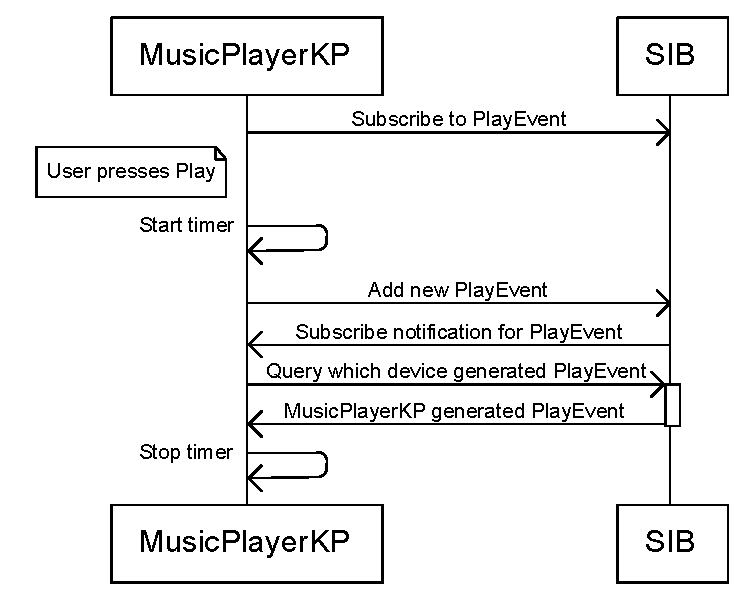
\includegraphics[width=200px]{n900}
\caption{Sequence diagram of Music Player KP subscription measurement}
\label{N900}
\end{figure}

\begin{figure}
\centering
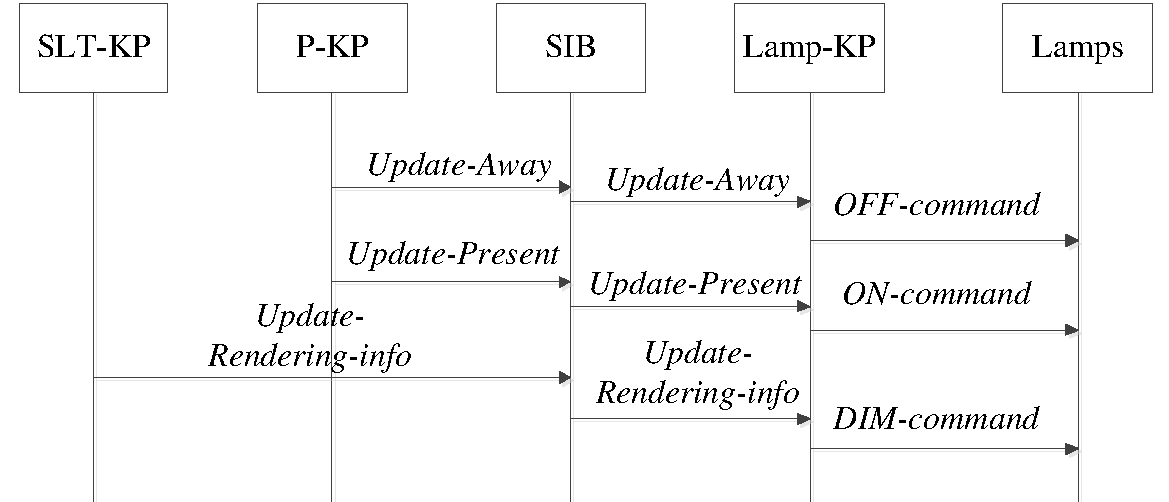
\includegraphics[width=200px]{sequence-lamp}
\caption{Sequence diagram of Presence-KP and Lamp-KP}
\label{sequence-lamp}
\end{figure}

\begin{figure}
\centering
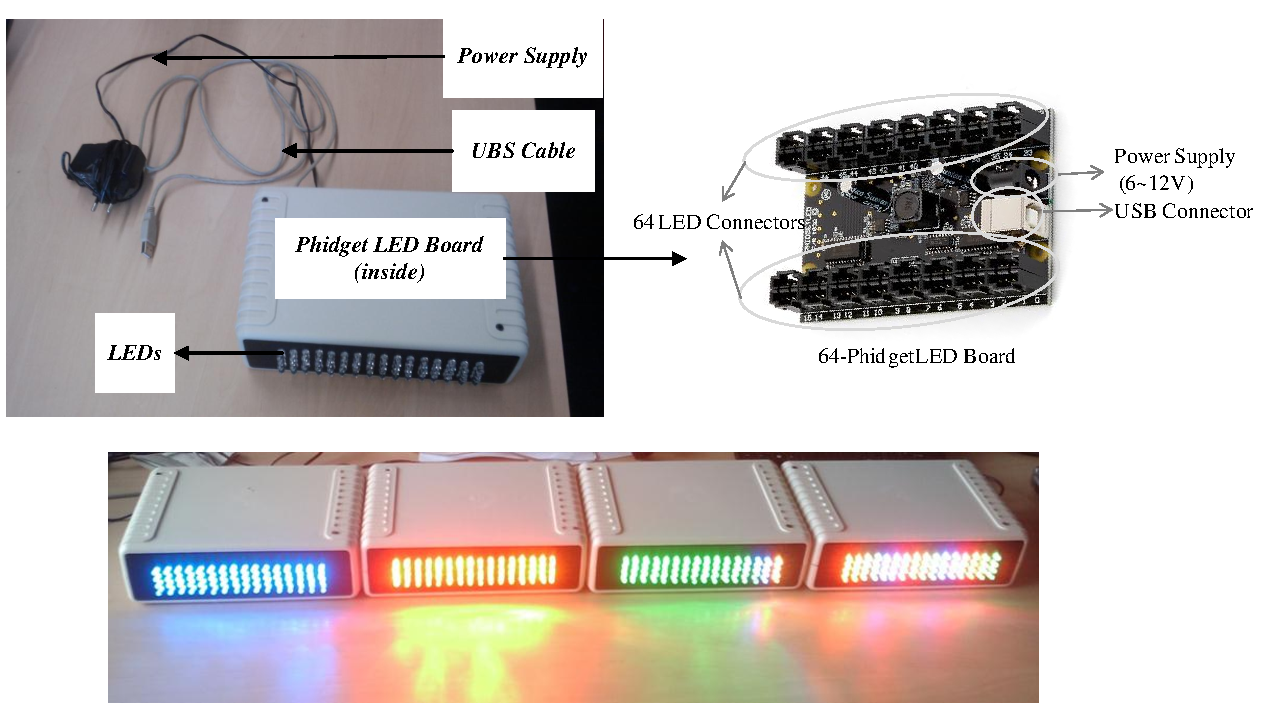
\includegraphics[width=250px]{lamp-KP}
\caption{Lamp-KP}
\label{lamp-KP}
\end{figure}

\subsubsection{Performing reasoning with the SIB}

Reasoning on information contained within the SIB was performed using OWL 2 RL and SPIN (See Section \ref{SPIN}).  OWL inferences for OWL 2 RL were executed by using SPIN rules. For more information on OWL 2 RL and SPIN, see Section \ref{owl2rl}.

When the SPIN engine is started (we use the open source TopBraid SPIN API), it iterates until there are no new triples constructed - we call this one \emph{reasoning cycle}. Existing inferences from a previous reasoning cycle are cleared before each new reasoning cycle. Triples that were previously inferred (based on a CONSTRUCT SPIN rule), are removed when the asserted triple (which caused the inferred triple) does not exist anymore. Triples are inferred (using SPIN rules) when new triples are inserted by devices connected to a triple store. For example, consider a device inserting a \texttt{sc:connectedTo} relationship when it is connected to another device. When the asserted triples are later removed by these devices (e.g. a device removing its \texttt{sc:connectedTo} relationship when the other device disconnects), the triples that were inferred based on these triples should be removed as well.

For the pilot, constraint violation checking was disabled, as this introduced quite a large delay ($>1000ms$), and was not necessary for the purposes of the pilot. Constraint checking ensures that instances in the triple store meet the constraints attached to classes and properties in an ontology. Constraint violation checks are computationally expensive and cannot be performed for each add, remove and update operation. One possible solution is to perform constraint violation checks at regular intervals and then remove the offending triples.

\subsubsection{OWL 2 RL and SPIN}
\label{owl2rl}

An example of where an OWL 2 property chain is used to perform semantic matching of media types is shown as:\\


\noindent
transmitsMediaType~\ensuremath{\circ}~isAcceptedMediaTypeOf\\~\ensuremath{\sqsubseteq}~convertsMediaType\footnote{The concatenation of two relations $R$ and $S$ is expressible by $R \circ S $, while $ R \sqsubseteq S$ indicates that $R$ is a subset of $S$ }\\


This is modelled in the ontology as:
\usemintedstyle{manni}
\begin{minted}[fontsize=\footnotesize]{turtle}
sc:convertsMediaType
	a owl:ObjectProperty; 
	a owl:IrreflexiveProperty ;
    owl:propertyChainAxiom
    	(sc:transmitsMediaType 
		 sc:isAcceptedMediaTypeOf) .
\end{minted}

% (moved to OntologyEngineering)
% We realized early on that some kind of rule-based functionality will be required in addition to the functionality provided by an ontology language like OWL 2. Originally we considered using SWRL (Semantic Web Rule Language) \cite{Niezen2011}, but it was deemed not expressive enough. Due to it being a DL (Description Logic)-safe language, it is not possible to create new individuals based on inferences. With SPARQL, this is possible using a CONSTRUCT query, defined as a SPIN rule as shown in Listing \ref{constructspin}.
% 
% 
% \begin{figure*} % \begin{listing} does not seem to support twocolumn
% % to use sparl lexer, install https://github.com/gniezen/n3pygments	
% \begin{minted}[linenos,
%                numbersep=5pt,
%                %gobble=2,
%                frame=lines,
%                fontsize=\footnotesize,
%                framesep=2mm]{sparql} 
% CONSTRUCT {
%     ?mp a sc:MediaPath .
%     ?x3 sc:hasMediaPath ?mp .
%     ?mp bonding:mediaSourceSO ?x2 .
%     ?mp bonding:mediaOriginator ?this .
% }
% WHERE {
%     ?this sc:convertsMediaType ?x2 .
%     ?x2 sc:convertsMediaType ?x3 .
%     ?this sc:connectedTo ?x3 .
%     BIND (IRI(fn:concat("example.com/ontology#mediaPath_", afn:localname(?this),
%      "_to_",afn:localname(?x3))) AS ?mp) .
% }
% \end{minted} 
% \captionof{listing}{Creating a new individual using SPARQL CONSTRUCT and SPIN} 
% % see http://tex.stackexchange.com/a/12430/8419
% \label{constructspin}
% \end{figure*}
% 
% In the example, a new \texttt{mediaPath} individual is created if two smart objects are connected to each other and there is a \texttt{mediaSourceSO} (semantic transformer) that converts the media types between them. This could be a media player transmitting music as source, an ambient lighting object that accepts RGB colour values as sink, and a semantic transformer that converts audio streams into RGB lighting information. For more information about media paths and semantic transformers, see \cite{Niezen2011}.
% 
% The \texttt{?this} variable indicates to SPIN how the definition should be applied to the members of a class, as the rule itself is defined as part of the class definition - thus defining the scope of the query. \texttt{fn:concat} and \texttt{afn:localname} are SPIN functions used to concatenate the name of the individual and retrieve the local names of the variables used respectively.

% Although SWRL is supported by the Pellet and HeRMiT reasoners, it is not yet standardized and has stayed a W3C Member Submission\footnote{http://www.w3.org/Submission/SWRL/} since 2004. SPARQL is a W3C Recommendation, actively developed and well supported by the Semantic Web community.

We made use of OWL 2 RL/RDF Rules, which is a \emph{semantic} subset of OWL 2 \emph{Full}. This should not be confused with the first part of the OWL 2 RL Profile\footnote{http://www.w3.org/TR/owl-profiles/}, which is a \emph{syntactic} subset of OWL 2 \emph{DL}, and restricted in the type of inferences that can be performed. In practice, most OWL 2 reasoners implement OWL 2 RL/RDF Rules (from here on known as OWL 2 RL). OWL 2 RL addresses a significant subset of OWL 2, including property chains and transitive properties. It is fully specified as a set of rules - in our case, as a set of SPIN rules\footnote{ http://topbraid.org/spin/owlrl-all}. This means that it is even possible to select only the parts of OWL 2 that are required for a specific ontology, to allow for scalable reasoning.
% Could add info about tractability

\subsubsection{Smart Space Access Protocol}

KPs communicate with the SIB through SSAP (Smart Space Access Protocol) messages \cite{Honkola2010} over TCP/IP. SSAP consists of a number of operations to insert, update and subscribe to information in the SIB. These operations are encoded using XML. During the smart home pilot, all SSAP messages received by the SIB were logged for further analysis.

\subsection{Experimental Results}
\label{results}

After every reasoning cycle both the asserted and inferred models were written to disk, generating a total of 8306 models during the pilot. Reasoning was performed once, after all ontologies were loaded, and then for every add, remove and update operation. This resulted in a total of 5158 measurements of model size and reasoning time during the pilot. No reasoning was performed during queries.

During the pilot, 70655 total queries were performed by devices connected to the SIB. The time to perform each query was recorded on the SIB, and is shown in Figure \ref{querytime}. The histogram with bin size 25 is plotted on a logarithmic scale. Around 70000 queries take 2ms or less to complete, accounting for more than 99\% of the queries. Of all the queries, only 3 queries took 30ms or longer to complete, with all queries completing in less than 60ms. Keep in mind that these measurements were performed on the SIB, hence it does not take network latency into account.

\begin{figure}
\centering
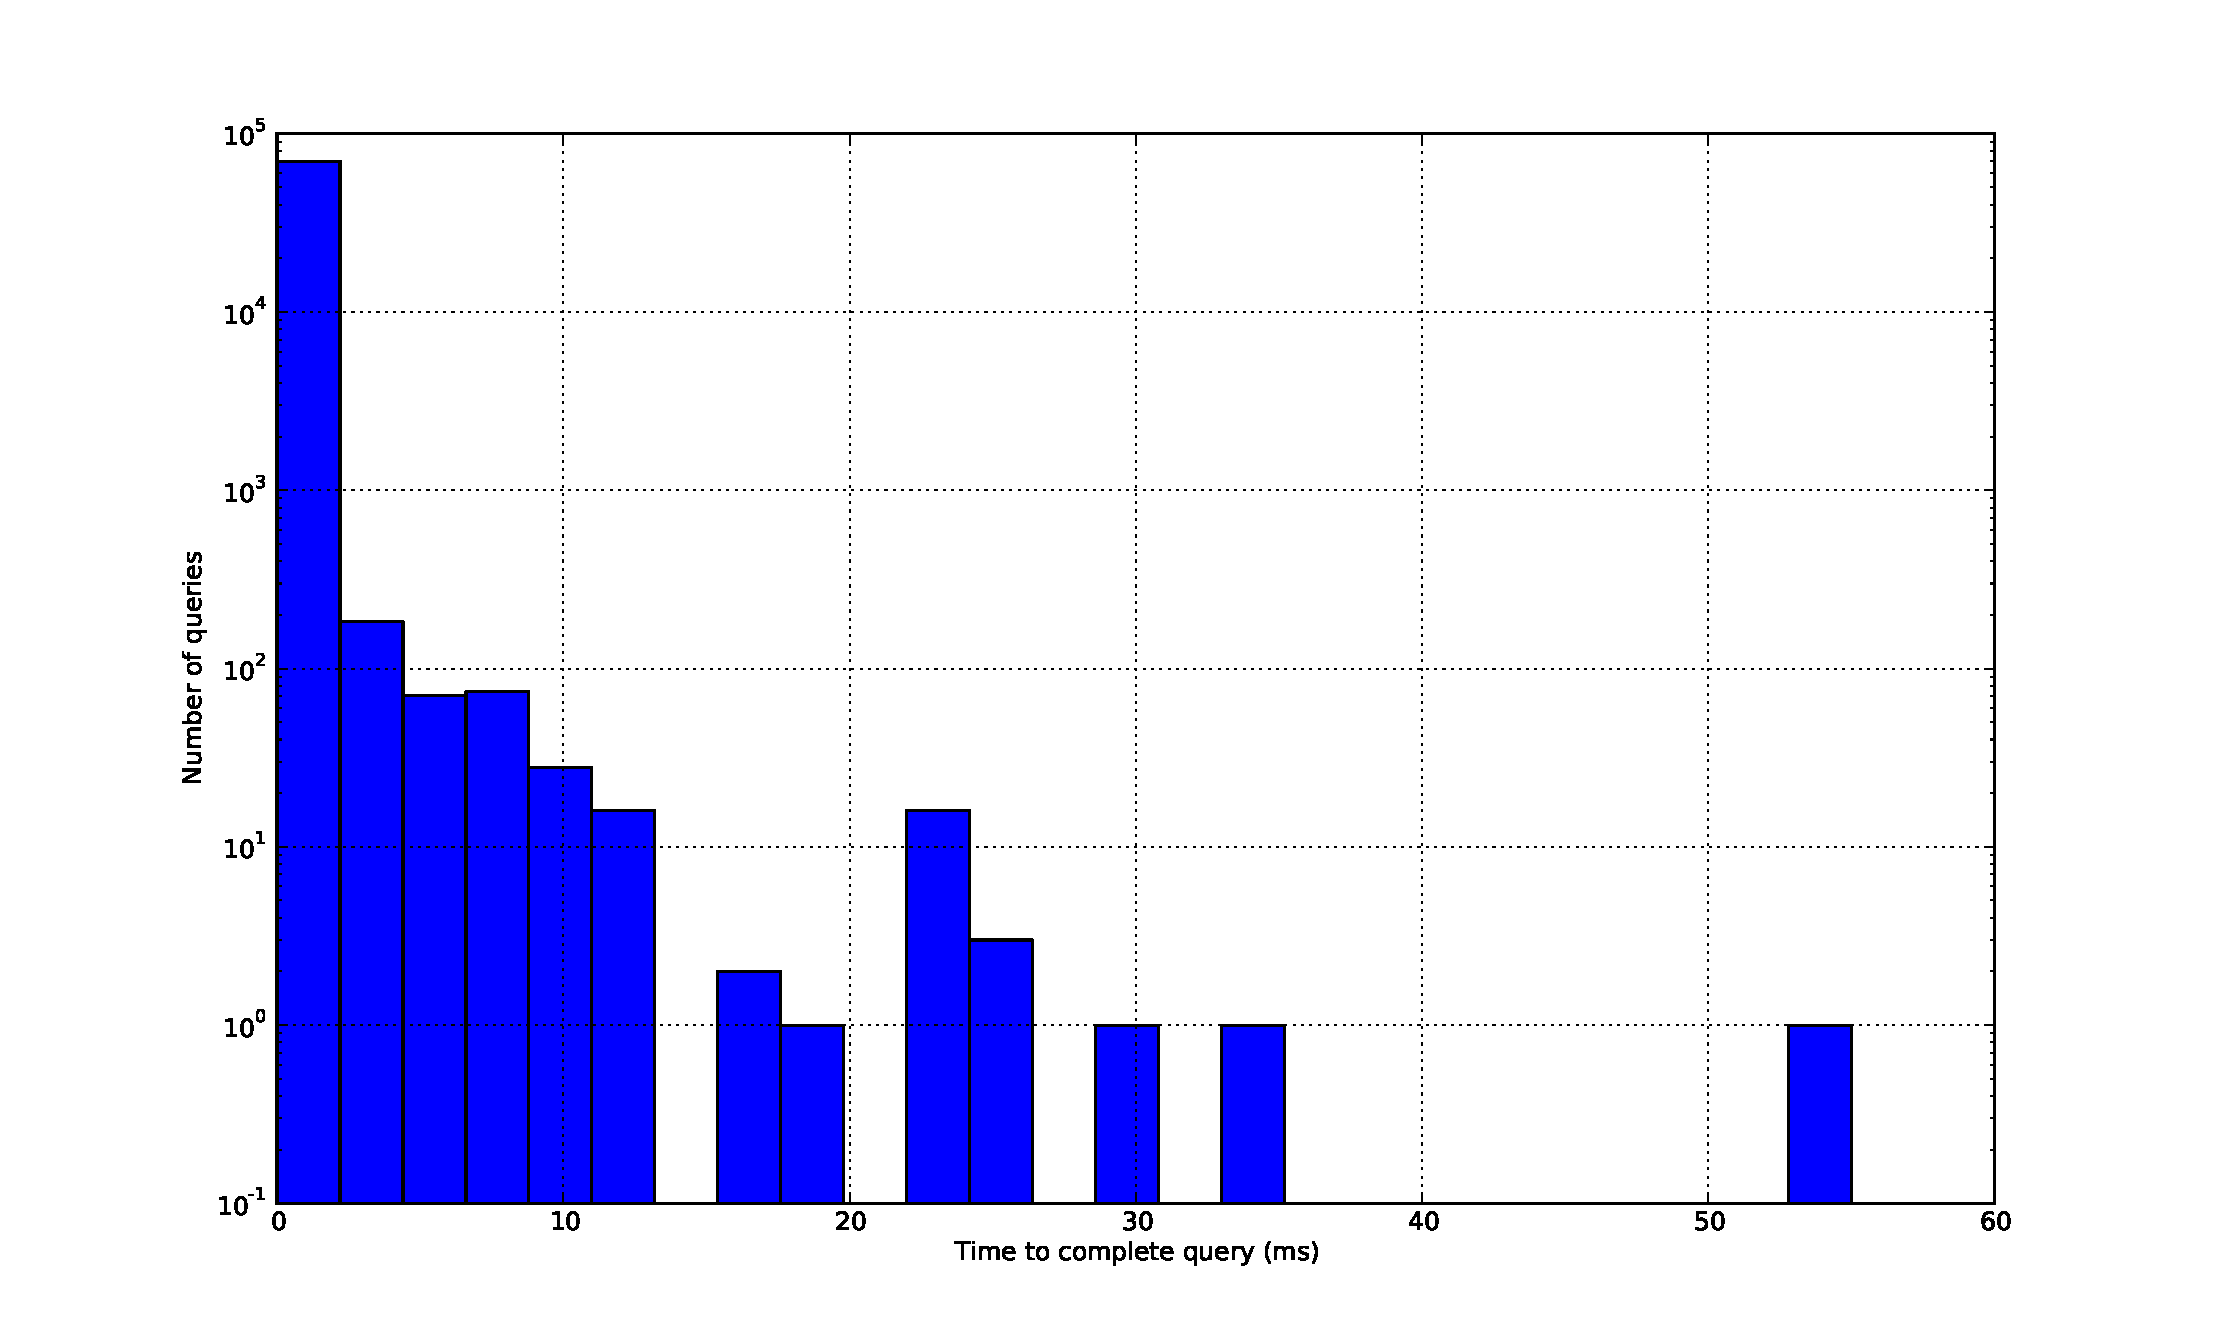
\includegraphics[width=250px]{querytime}
\caption{Query time measurements on SIB}
\label{querytime}
\end{figure}

Figure \ref{kdeplot} shows the histograms, Gaussian kernel density estimates (KDEs) and cumulative distribution functions (CDFs) of the Connector KP and Sound/Light Transformer KP \emph{query time measurements}. A bin size of 20 and a bandwidth of 0.5 was used to plot the figures. It shows that the typical query time for the Connector KP is very short, with a few outliers that took a very long time to complete (35.2s). For the SLT KP, the case is similar, but there are no extreme outliers, with the longest query taking only 587ms to complete. Note that the KDE provides similar information to the histogram, but handles outliers more gracefully by not using binning, and also results in a smoother graph.

The CDF of the Connector KP indicates that queries taking more than 2 seconds to complete are very rare, but the ones that do take an unusually long time to complete. We believe that it could be related to problems in the wireless network, or related to the Python implementation of the Knowledge Processor Interface (KPI), as the problem did not present itself when using other KPI implementations.

For the SLT KP, most queries completed within 100ms, with very few queries taking longer than 500ms to complete.

\begin{figure}
\centering
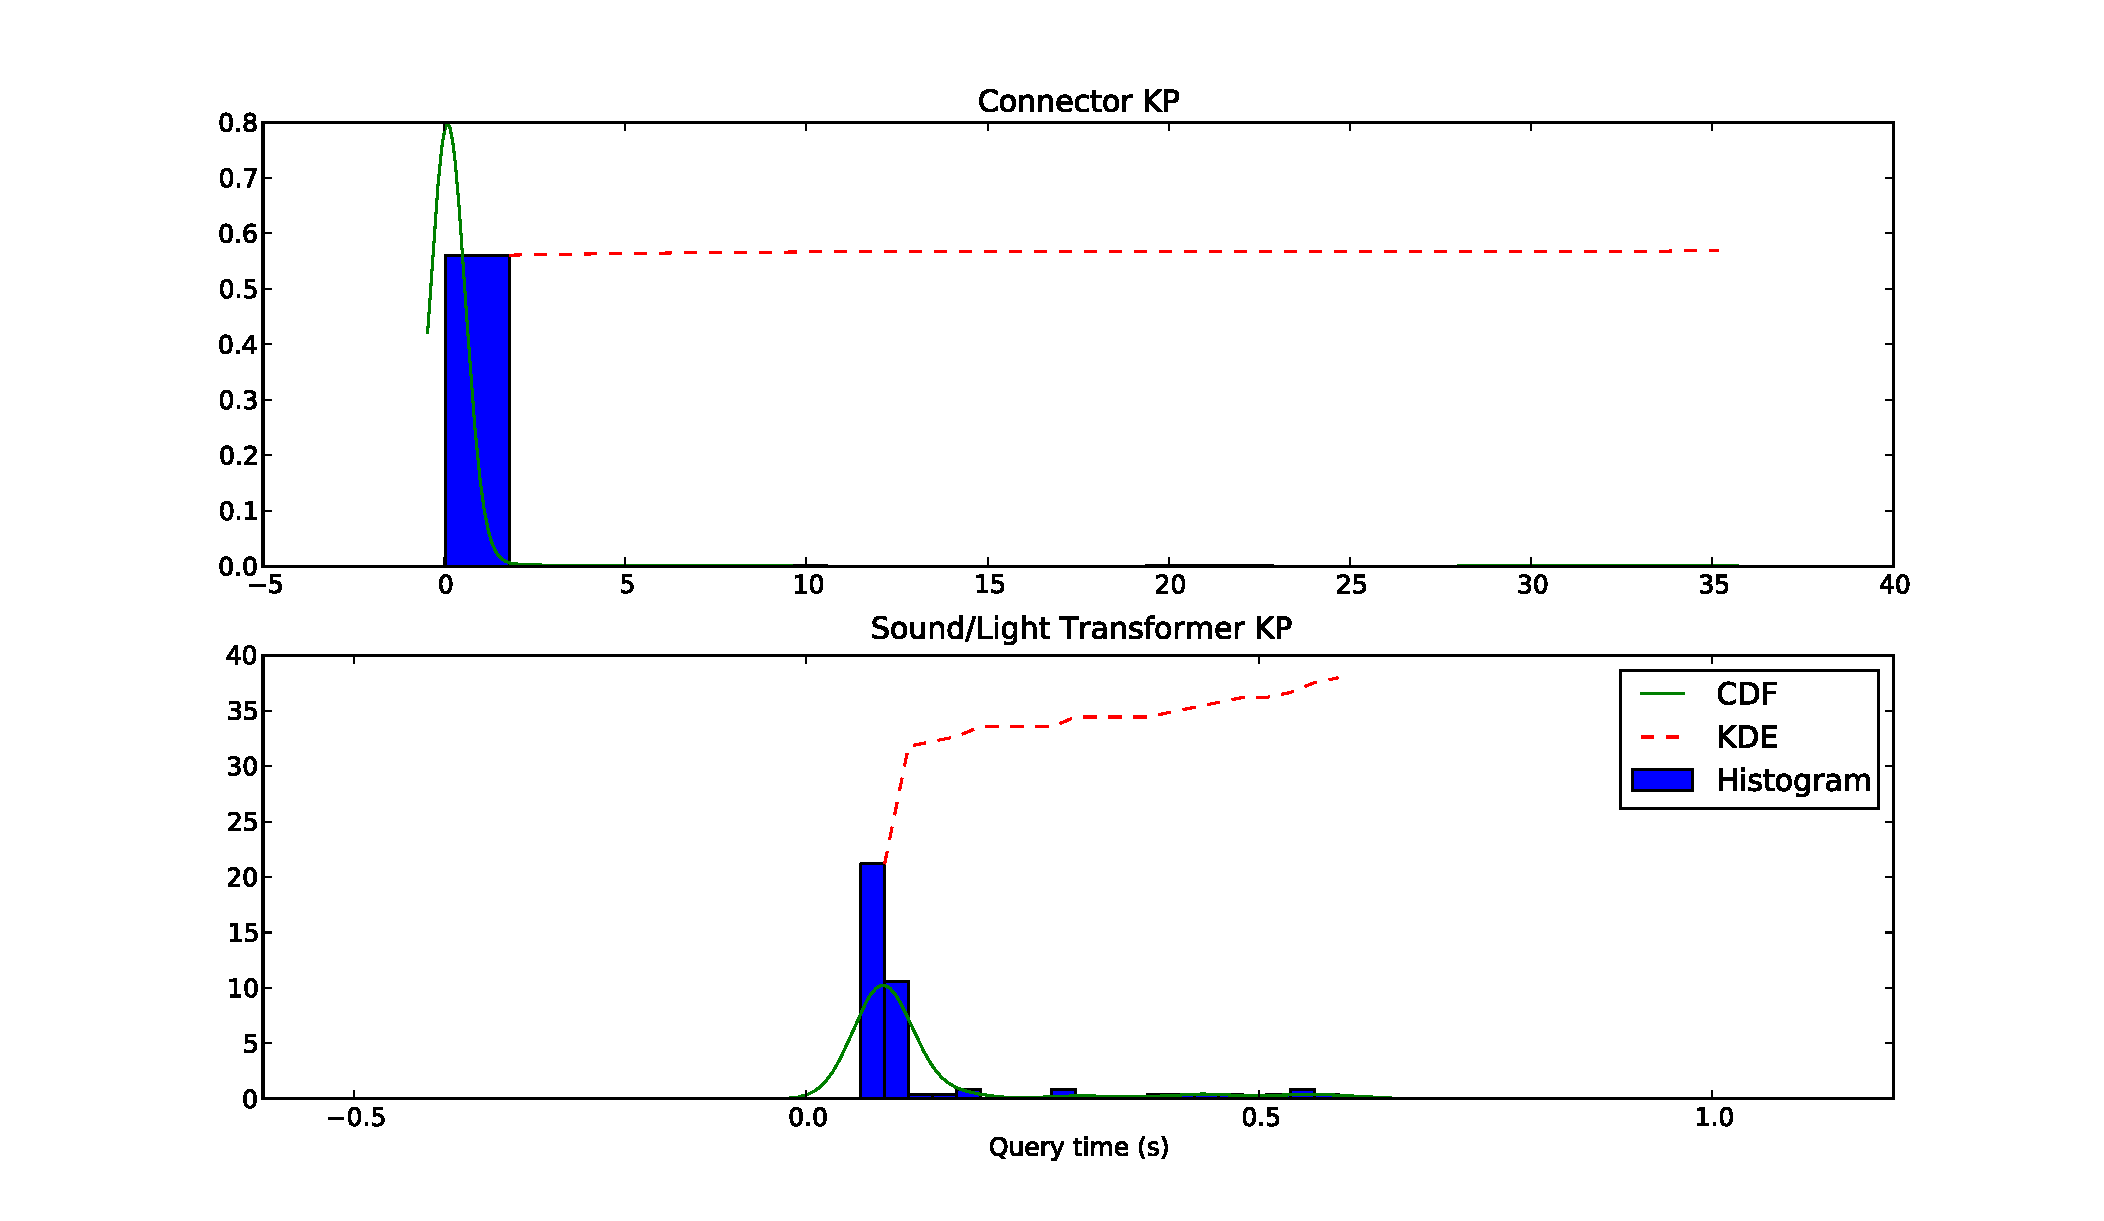
\includegraphics[width=250px]{kdeplot}
\caption{Histograms, kernel density estimates and cumulative distribution functions of Connector KP and Sound/Light Transformer KP measurements}
\label{kdeplot}
\end{figure}

For the music player KP, most subscription notifications completed in an average of 0.86s, as shown in Figure \ref{n900plot}. Keep in mind that after the new PlayEvent is added, inferencing is performed on the triple store before the subscribe notification is generated. Summary statistics of Music Player KP, Connector KP and Sound/Light Transformer KP measurements are shown in Table \ref{summaryKP}.

\begin{figure}
\centering
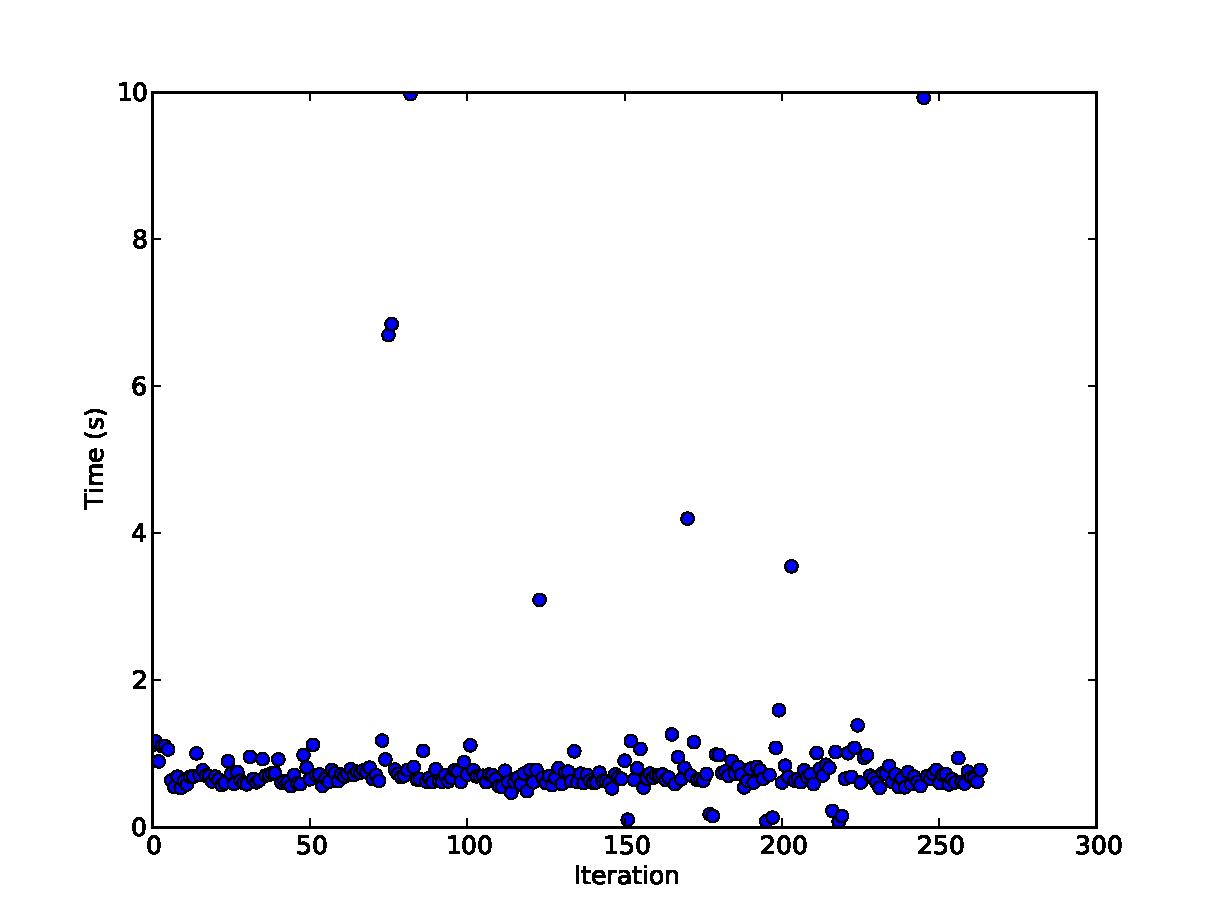
\includegraphics[width=250px]{n900plot}
\caption{Subscription measurements of Music Player KP}
\label{n900plot}
\end{figure}

\begin{table}[!t]
\caption{Summary statistics of Music Player KP, Connector KP and Sound/Light Transformer KP measurements}
\label{summaryKP}
\centering
\begin{tabular}{|l|l|l|l|l|l|}
\hline
Component &	 Nr. of obs. & Min. & Max. & Mean &	Std. dev.\\
\hline
Music Player KP & 264 & 0.074 & 9.975 & 0.861 & 1.017\\
Connector KP & 961 & 0.044 & 35.184 & 0.275 & 1.942\\
Sound/Light KP  & 86 & 0.06 & 0.587 & 0.131 & 0.122 \\
Lamp-KP & 98 & 0.012 & 0.049 & 0.03 &0.006 \\
Presence-KP & 172 & 0.145 & 0.244 & 0.176 & 0.018 \\
\hline
\end{tabular}
\end{table}

In Figure \ref{stats}, the following is shown:
\begin{itemize}
\item Model size: Number of triples asserted by ontology or connected KPs
\item Inferred model size: Number of triples inferred by reasoning engine
\item Inferencing duration: Time (in ms) to complete one reasoning cycle
\end{itemize}

The sharp peaks indicate the times that the SIB was restarted. The first reasoning cycle after a restart takes about 3 seconds,  with subsequent cycles taking on average 275ms (as seen in Table \ref{summarySIB}).

There is a slow but steady increase in the number of triples as new events get added to the triple store. After each restart these events are cleared and the base assertions loaded from the ontology. These assertions include the OWL 2 RL specification, stored as SPIN rules, which account for the large number of triples.

\begin{figure}
\centering
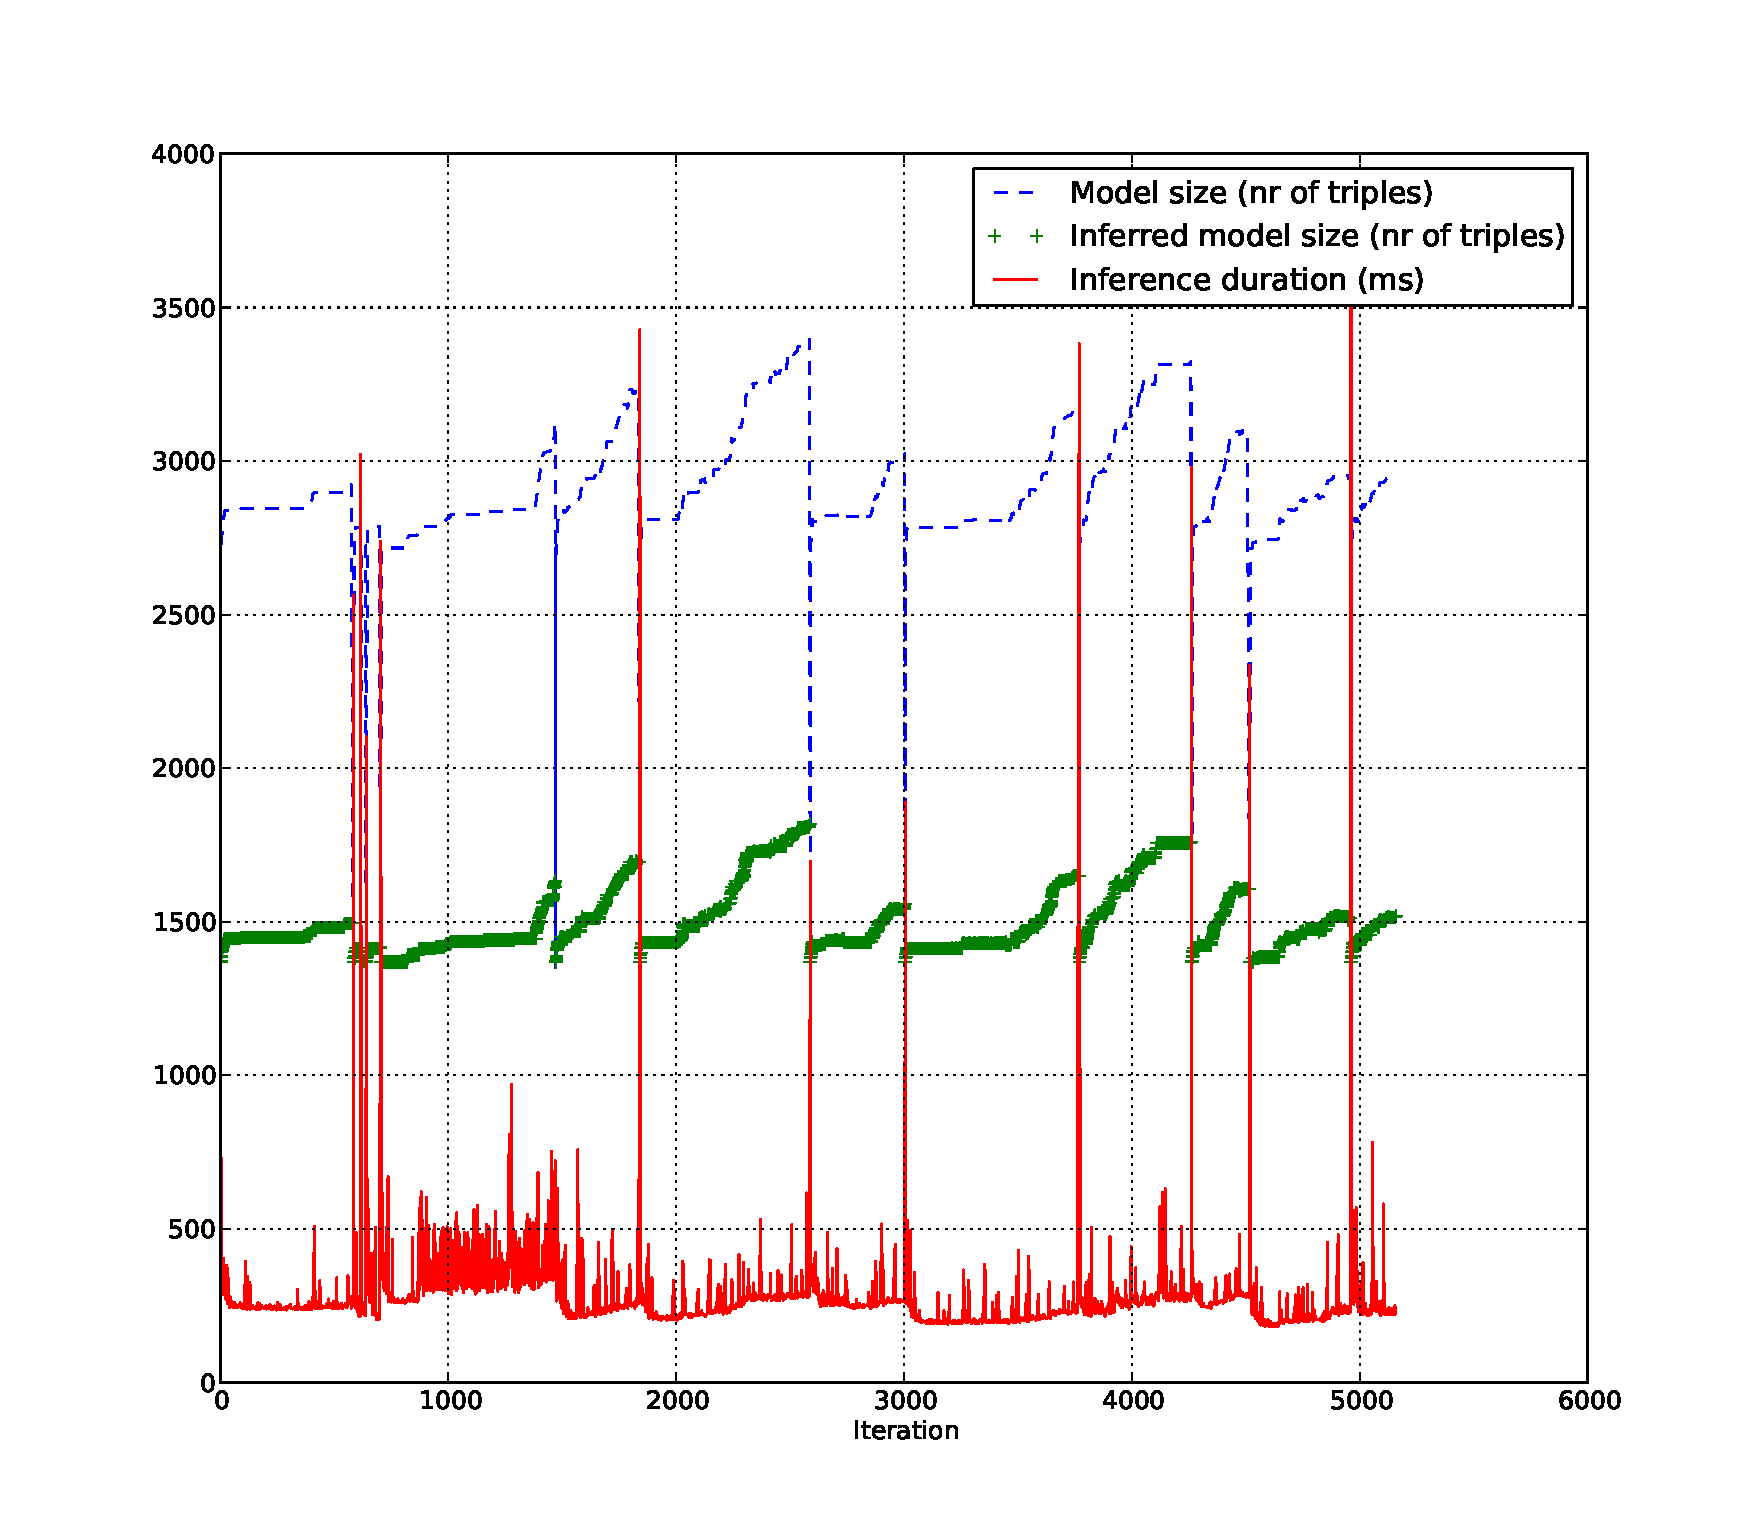
\includegraphics[width=250px]{stats}
\caption{Size of asserted and inferred models for each iteration, including reasoning time}
\label{stats}
\end{figure}

\begin{table}[!t]
\caption{Summary statistics for asserted and inferred model sizes and reasoning time}
\label{summarySIB}
\centering
\begin{tabular}{|l|l|l|l|l|l|}
\hline
Component &	 Nr. of obs. & Min. & Max. & Mean &	Std. dev.\\
\hline
Model size	& 5158 & 1346 &	3396 &	2916.7 & 201.07 \\
Inferred model size &	5158 &	1369 &	1819 &	1501.8 & 107.6 \\
Reasoning time & 5158 &	181 & 2912 & 274.99 & 152.96 \\
\hline
\end{tabular}
\end{table}

In Figure \ref{CPD}, the measurements show that the delay between the P-KP and the SIB is rather large with a considerable variance. The communication from the P-KP to the SIB consists of an update request and the related confirmation response. The average delay of 176.71 milliseconds is the largest component of the total end-to-end delay between the links. The communication from the SIB to the Lamp-KP consists of an indication event from the SIB due to a subscription and results in a query request from the Lamp-KP, terminated by a confirmation response by the SIB. There is some variance in the communication delay and the average delay of 25.87 milliseconds might become problematic when the SIB has to inform and handle multiple subscribers.

\begin{figure}
\centering
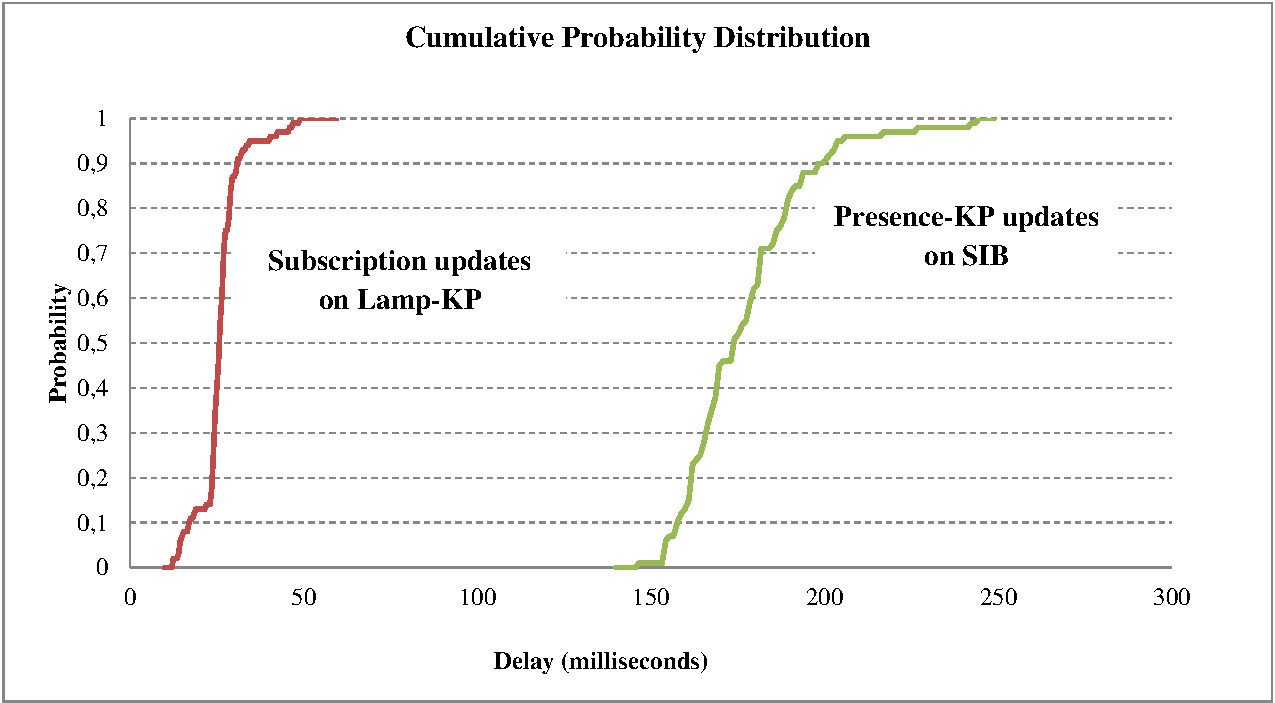
\includegraphics[width=250px]{CPD}
\caption{Cummulitive probability distribution of delays between Presence-KP and SIB, and SIB and Lamp-KP}
\label{CPD}
\end{figure}

\subsection{Discussion}

During the pilot, most problems could be attributed to problems with the wireless network. A number of devices from different manufacturers experienced intermittent problems while connected to the SIB. For the purposes of the pilot, these devices were then connected to the SIB via ethernet. This does, however, demonstrate some of the problems with existing wireless networking technologies. It cannot be expected that a device with a wireless connection will always stay connected to the smart space, even when it is within range of the wireless router.

%During one stakeholder visit, the comment was made that what we term semantic transformers, could also be termed transcoders, as they transcode data from one source type to another. With a large number of stakeholder visits the similarities of the SOFIA system to Universal Plug \& Play (UPnP) were discussed. It was pointed out that uPnP only covers one domain, and that it does not allow for the same type of device and capability descriptions on the semantic level.

If we compare our query time measurements to the ones performed on Smart-M3 (4.4ms) and RIBS (0.65ms), we can see that the KPs were substantially slower: The Connector KP at 44ms, the Music Player KP at 74ms and the Sound/Light KP at 60ms. This can be attributed to additional network latency in the field study that approximated a real-world environment. Query measurements that were performed on the ADK-SIB directly (0.445ms) shows that it performs even better than RIBS, but this is not directly comparable as it does not include network latency time. If network latency is taken into account, measured at 0.43ms per packet round-trip by \cite{Etelapera2011}, RIBS is still faster.

The subscription indication measurements of our setup are also significantly slower. While the Smart-M3 measurement was only 140ms, the Music Player KP measures around 860ms. This is mostly due to the additional time required for reasoning, which on average takes about 275ms. Other contributing factors include the number of devices used, the number of triples and the network environment.

In the 1960s there already existed some controversy over the maximum allowable response times in human-computer interfaces \cite{Miller1968}. It was shown that different human actions will have different acceptable response times. While the delay between pressing a key and visual feedback should be no more than 0.1-0.3 seconds, the response to a inquiry request may take up to 2 seconds. The performance measurements are still well within this two-second limit, indicating that from a user's point of view, when performing routine tasks, the system is responsive enough. The user study and interviews performed during the pilot seem to confirm this, as no participant indicated any issues with regards to the responsiveness of the system.

The scalability of the system should still be evaluated with larger triple sizes, but we do not foresee any scalability issues, due to the platform and software architecture used. 

%When addressing another human being, we expect some communicative response between two and four seconds - any longer delay breaks the thread of communication and becomes embarrassing.


%SeNAmI end


\section{Evaluating the ontology}

A variety of methods have been proposed \cite{DAquin2011} to evaluate ontology quality:

\begin{itemize}
	\item Testing and assessing the formal properties, e.g. using OntoClean (see Section TODO)
	\item Using ontology design patterns (see Section \ref{DesignPatterns})
	\item Using unit tests as employed in software engineering
	\item Using opinions and rating using crowd-sourcing
	\item Using automatically generated metrics
\end{itemize}

In the book Beautiful Data \cite{Segaran2009}, the notion of beauty is described as ``a simple and elegant solution to some kind of problem''. In a paper on the notion of beauty when building and and evaluating ontologies, D'Aquin and Gangemi \cite{DAquin2011} argue that the GoodRelations\footnote{http://www.heppnetz.de/projects/goodrelations/} e-commerce ontology could be considered an example of a beautiful ontology. It addresses a complex domain and covers many of the complex situations that can occur in the domain. It is well designed, ontologically consistent, lightweight and used extensively by practitioners in the domain. GoodRelations is an OWL 1 DL ontology that is used by stores to describe products and their prices and features. Companies using the ontology include, Google, BestBuy, Sears, K-Mart and Yahoo.

Hepp \cite{Hepp2007} describes a number of characteristics that can be used to evaluate an ontology:

\begin{itemize}
	\item Expressiveness: An ontology of higher expressiveness would be richly axiomatised in higher order logic, while a simple vocabulary would be of low expressiveness.
	\item Size of community: As ontologies are considered community contracts (see Section \ref{CommunityContract}), an ontology targeted towards a large community should be easy to understand, well documented and of a reasonable size.
	\item Number of conceptual elements: A larger ontology is more difficult to visualise and review. A reasoner could also take a long time to converge when the ontology is very large.
	\item Degree of subjectivity: This is very much related to the domain of the ontology, where something like religion would be more subjectively judged than engineering.
	\item Average size of specification per element: The number of axioms or attributes used to describe each concept influences the ontological commitment\label{OntologicalCommitment} that must be made before adopting the ontology. \marginpar{Ontological commitment relates to \emph{premature commitment}, which is described in more detail in Section TODO on the Cognitive Dimensions framework.}
\end{itemize}








TODO Compare with DLNA/UPnP as a case study

Possible TODO
Compare to Logitech Harmony One Universal Remote Control (See Evernote)
- Compare ontological approach to APIs http://itu.dk/stud/speciale/gamelib/APIUsability.pdf
- Validate generalization of ontology (compared to existing ones)